\scanpage{12}
Les conditions a) b) c) sont les \uline{conditions logiques} élémentaires. On veut de plus

\margin{c) puis d) (condition différentielle)}
\unsure{d)|e)} (Condition hensélienne) Si $u:X_n\mathbin{-}X_n$ est un $A_*$-morphisme qui est un isomorphisme formel (i.e. si $f_1,\ldots,f_n\in A_n$ sont tels que $\varepsilon(f_1)\ldots\varepsilon(f_n)$ sont nilpotents dans $k$ et
\[
\varepsilon\left(\det\left(\frac{\partial f_i}{\partial\unsure{t_j|x_j}}\right)\right)
=\det\left(\varepsilon\left(\frac{\partial f_i}{\partial x_j}\right)\right)
=\det\left(\frac{\partial f_i}{\partial x_j}(0)\right)
\]
est un élément inv. de $k$) alors $u^{-1}$ est aussi un $A_*$-morphisme ($\Leftrightarrow$ le foncteur des $A_*$-schémas $A_*$ formels vers les schémas formels sur $k$ est conservatif).

\uline{Cor. 1} Si $f\in A_n$ et $f$ inversible dans $S_n$, i.e. $\varepsilon(f)=f(0)$ inversible dans $k$, alors $f^{-1}\in A_n$; \deleted{\unsure{f inversible|f même inversible}} si $f\in A_n$, $\varepsilon(f)=0$, alors $(1+f)^{-1}\in A_n$ ($\Leftrightarrow$ si $f\in A_n$ et $\varepsilon(f)=1$, alors $f^{-1}\in A_n$) $\Leftrightarrow A_n\cap\mathfrak m_n\subset\operatorname{rad}A_n$, où \deleted{$\unsure{\mathfrak m_n=}$} $\mathfrak m_n=(t_1,\ldots,t_n)S_n$ \deleted{\unsure{cas nilpotent de l'élément}}.
\margin{moyennant condition d) (différentielle)}

En effet, considérons le \deleted{\unsure{multi}} morphisme
\[
u:(x_1,\ldots,x_n,x_{n+1})\longmapsto
(x_1,\ldots,x_n,f(x_1,\ldots,x_n).x_{n+1})
\]
de $X_{n+1}$, il est un isom. formel d'inverse
\[
(x_1,\ldots,x_n,x_{n+1})\longmapsto
(x_1,\ldots,x_n,f(x_1,\ldots,x_n)^{-1}x_{n+1}),
\]
et comme \deleted{il} \inserted{$u$} est un $A_*$-morphisme, par d) il en est de $=$ de $u^{-1}$, donc
\[
g(t_1,\ldots,t_{n+1})=f(t_1,\ldots,t_n)^{-1}t_{n+1}\in A_{n+1},
\]
\deleted{i.e. $X_{n+1}\mathbin{-}X_1$ \unsure{comme}} donc $g(t_1,\ldots,t_n,1)\in A_n$ i.e. $f^{-1}\in A_n$. cqfd.
\margin{\unsure{ridicule avec la condition différentielle}}
\margin{incorrect, 1 n'est pas nilp.! Il faut exiger une propriété de divisi-bilité
\[
t_{n+1}f\in A_{n+1}\Longrightarrow f\in\unsure{A_{n+1}|A_n}
\]}
\figure{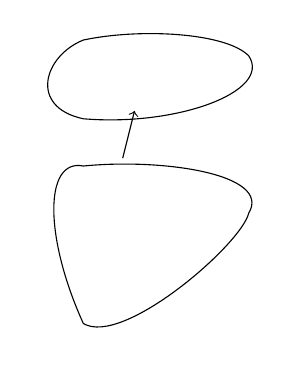
\begin{tikzpicture}[x=1cm,y=1cm]\draw (0,0) .. controls (-.7,.15) and (-.5,.8) .. (0,1) .. controls (.7,1.15) and (1.8,1.1) .. (2.1,.8) .. controls (2.4,.35) and (1.2,-.1) .. (0,0);\draw[->] (.5,-.5)--(.65,.1);\draw (0,-.6) .. controls (-.5,-.5) and (-.5,-1.5) .. (0,-2.6) .. controls (.5,-2.9) and (2,-1.6) .. (2.1,-1.2) .. controls (2.4,-.7) and (1,-.5) .. (0,-.6);\end{tikzpicture}}

\uline{Cor. 2} Soit \inserted{$P(Z)=$} $Z^N+f_1Z^{N-1}+\cdots+f_N\in A_n[Z]$ polynôme unitaire, soit $\zeta\in k_0$ tel que
\[
P^\varepsilon(\zeta)=\zeta^N+a_1\zeta^{N-1}+\cdots+a_N=0,
\quad\text{où les }a_i=\varepsilon(f_i)=f_i(0)\in k_0,
\]
\mspage{11}
